\def \root {../../}			% path to root (/notes)
\documentclass[11pt, oneside]{article}   	% use "amsart" instead of "article" for AMSLaTeX format
\usepackage[margin = 1in]{geometry}                		% See geometry.pdf to learn the layout options. There are lots.
\geometry{letterpaper}                   		% ... or a4paper or a5paper or ... 
%\geometry{landscape}                		% Activate for rotated page geometry
%\usepackage[parfill]{parskip}    		% Activate to begin paragraphs with an empty line rather than an indent
\usepackage{graphicx}				% Use pdf, png, jpg, or eps§ with pdflatex; use eps in DVI mode
								% TeX will automatically convert eps --> pdf in pdflatex		
\usepackage{amssymb}
\usepackage{amsmath}
\usepackage[shortlabels]{enumitem}
\usepackage{float}
\usepackage{tikz-cd}
\usepackage{subcaption}
\usepackage{simpler-wick}
\usepackage[compat=1.0.0]{tikz-feynman}   %note you need to compile this in LuaLaTeX for diagrams to render correctly

\usepackage{verbatim}
\usepackage{amsthm}
\usepackage{hyperref}

%%%%%%%%%%%%%%%%%%%%%%%%%%%%%%%%%%%%%%%%%%%%%%%%
%%%%%%%%%%%%%%% CUSTOM MATH ENVIRONMENTS %%%%%%%%%%%%%%%
%%%%%%%%%%%%%%%%%%%%%%%%%%%%%%%%%%%%%%%%%%%%%%%%

\usepackage{mdframed}
\usepackage{xparse}
\usepackage{framed}		% Colored boxes. \begin{shaded} to use the package
\usepackage{minted}

\definecolor{lightgray}{rgb}{0.93, 0.93, 0.93}
\definecolor{lightpurple}{rgb}{0.9, 0.7, 1.0}
\definecolor{lightblue}{rgb}{0.2, 0.7, 0.7}
%\definecolor{lightred}{rgb}{0.8, 0.2, 0.2}
\definecolor{lightred}{rgb}{0.99, 0.0, 0.0}
\definecolor{lightgreen}{rgb}{0.2, 0.6, 0.2}
\definecolor{magenta}{rgb}{0.9, 0.2, 0.9}

\colorlet{shadecolor}{lightgray}		% 40% purple, 40% white
\colorlet{defcolor}{lightpurple!40}
\colorlet{thmcolor}{lightblue!20}
\colorlet{excolor}{lightred!30}
\colorlet{rescolor}{lightgreen!40}
\colorlet{intercolor}{magenta!40}

% Definition
\newcounter{dfnctr}
\newenvironment{definition}[1][]{
\stepcounter{dfnctr}
%\protected@edef\@currentlabelname{dfnctr}
\ifstrempty{#1}
{\mdfsetup{
frametitle={
\tikz[baseline=(current bounding box.east),outer sep=0pt]
\node[anchor=east,rectangle,fill=defcolor]
{\strut Definition~\arabic{dfnctr}};}}
}
{\mdfsetup{
frametitle={
\tikz[baseline=(current bounding box.east),outer sep=0pt]
\node[anchor=east,rectangle,fill=defcolor]
{\strut Definition~\arabic{dfnctr}:~#1};}}
}
\mdfsetup{innertopmargin=3pt,linecolor=lightpurple,
linewidth=2pt,topline=true,
frametitleaboveskip=\dimexpr-\ht\strutbox\relax,}
%\begin{mdframed}[skipabove=2cm, splittopskip=\baselineskip]\relax%
\begin{mdframed}[]\relax%
}{\end{mdframed}}

% Theorem
\newcounter{thmctr}
\newenvironment{theorem}[1][]{
\stepcounter{thmctr}
\ifstrempty{#1}
{\mdfsetup{
frametitle={
\tikz[baseline=(current bounding box.east),outer sep=0pt]
\node[anchor=east,rectangle,fill=thmcolor]
{\strut Theorem~\arabic{thmctr}};}}
}
{\mdfsetup{
frametitle={
\tikz[baseline=(current bounding box.east),outer sep=0pt]
\node[anchor=east,rectangle,fill=thmcolor]
{\strut Theorem~\arabic{thmctr}:~#1};}}
}
\mdfsetup{innertopmargin=3pt,linecolor=lightblue!60,
linewidth=2pt,topline=true,
frametitleaboveskip=\dimexpr-\ht\strutbox\relax,}
\begin{mdframed}[]\relax%
}{\end{mdframed}}

% Corollary
\newcounter{corctr}
\newenvironment{corollary}[1][]{
\stepcounter{corctr}
\ifstrempty{#1}
{\mdfsetup{
frametitle={
\tikz[baseline=(current bounding box.east),outer sep=0pt]
\node[anchor=east,rectangle,fill=thmcolor]
{\strut Corollary~\arabic{corctr}};}}
}
{\mdfsetup{
frametitle={
\tikz[baseline=(current bounding box.east),outer sep=0pt]
\node[anchor=east,rectangle,fill=thmcolor]
{\strut Corollary~\arabic{corctr}:~#1};}}
}
\mdfsetup{innertopmargin=3pt,linecolor=lightblue!60,
linewidth=2pt,topline=true,
frametitleaboveskip=\dimexpr-\ht\strutbox\relax,}
\begin{mdframed}[]\relax%
}{\end{mdframed}}

% Proposition
\newcounter{propctr}
\newenvironment{prop}[1][]{
\stepcounter{propctr}
\ifstrempty{#1}
{\mdfsetup{
frametitle={
\tikz[baseline=(current bounding box.east),outer sep=0pt]
\node[anchor=east,rectangle,fill=thmcolor]
{\strut Proposition~\arabic{propctr}};}}
}
{\mdfsetup{
frametitle={
\tikz[baseline=(current bounding box.east),outer sep=0pt]
\node[anchor=east,rectangle,fill=thmcolor]
{\strut Proposition~\arabic{propctr}:~#1};}}
}
\mdfsetup{innertopmargin=3pt,linecolor=lightblue!60,
linewidth=2pt,topline=true,
frametitleaboveskip=\dimexpr-\ht\strutbox\relax,}
\begin{mdframed}[]\relax%
}{\end{mdframed}}

% Lemma
\newcounter{lemctr}
\newenvironment{lemma}[1][]{
\stepcounter{lemctr}
\ifstrempty{#1}
{\mdfsetup{
frametitle={
\tikz[baseline=(current bounding box.east),outer sep=0pt]
\node[anchor=east,rectangle,fill=thmcolor]
{\strut Lemma~\arabic{lemctr}};}}
}
{\mdfsetup{
frametitle={
\tikz[baseline=(current bounding box.east),outer sep=0pt]
\node[anchor=east,rectangle,fill=thmcolor]
{\strut Lemma~\arabic{lemctr}:~#1};}}
}
\mdfsetup{innertopmargin=3pt,linecolor=lightblue!60,
linewidth=2pt,topline=true,
frametitleaboveskip=\dimexpr-\ht\strutbox\relax,}
\begin{mdframed}[]\relax%
}{\end{mdframed}}

% Example
\newcounter{exctr}
\newenvironment{example}[1][]{
\stepcounter{exctr}
\ifstrempty{#1}
{\mdfsetup{
frametitle={
\tikz[baseline=(current bounding box.east),outer sep=0pt]
\node[anchor=east,rectangle,fill=excolor]
{\strut Example~\arabic{exctr}};}}
}
{\mdfsetup{
frametitle={
\tikz[baseline=(current bounding box.east),outer sep=0pt]
\node[anchor=east,rectangle,fill=excolor]
{\strut Example~\arabic{exctr}:~#1};}}
}
\mdfsetup{innertopmargin=3pt,linecolor=excolor,
linewidth=2pt,topline=true,
frametitleaboveskip=\dimexpr-\ht\strutbox\relax,}
\begin{mdframed}[]\relax%
}{\end{mdframed}}

% Resources
\newcounter{resctr}
\newenvironment{resources}[1][]{
\stepcounter{resctr}
\ifstrempty{#1}
{\mdfsetup{
frametitle={
\tikz[baseline=(current bounding box.east),outer sep=0pt]
\node[anchor=east,rectangle,fill=rescolor]
{\strut Resources};}}
}
{\mdfsetup{
frametitle={
\tikz[baseline=(current bounding box.east),outer sep=0pt]
\node[anchor=east,rectangle,fill=rescolor]
{\strut Resources};}}
}
\mdfsetup{innertopmargin=3pt,linecolor=rescolor,
linewidth=2pt,topline=true,
frametitleaboveskip=\dimexpr-\ht\strutbox\relax,}
\begin{mdframed}[]\relax%
}{\end{mdframed}}

% Interlude
\newcounter{interctr}
\newenvironment{interlude}[1][]{
\stepcounter{interctr}
\ifstrempty{#1}
{\mdfsetup{
frametitle={
\tikz[baseline=(current bounding box.east),outer sep=0pt]
\node[anchor=east,rectangle,fill=intercolor]
{\strut Example~\arabic{interctr}};}}
}
{\mdfsetup{
frametitle={
\tikz[baseline=(current bounding box.east),outer sep=0pt]
\node[anchor=east,rectangle,fill=intercolor]
{\strut Interlude~\arabic{interctr}:~#1};}}
}
\mdfsetup{innertopmargin=3pt,linecolor=intercolor,
linewidth=2pt,topline=true,
frametitleaboveskip=\dimexpr-\ht\strutbox\relax,}
\begin{mdframed}[]\relax%
}{\end{mdframed}}

%%%%%%%%%%%%%%%%%%%%%%%%%%%%%%%%%%%%%%%%%%%%%%%%
%%%%%%%%%%%%%%%%%% MATH COMMANDS %%%%%%%%%%%%%%%%%%%
%%%%%%%%%%%%%%%%%%%%%%%%%%%%%%%%%%%%%%%%%%%%%%%%

\usepackage{slashed}
\usepackage{bm}
\usepackage{cancel}

% Equation
\def\eq{\begin{equation}\begin{aligned}}
\def\qe{\end{aligned}\end{equation}}

% Common mathbb's
\newcommand{\N}{\mathbb{N}}
\newcommand{\R}{\mathbb{R}}
\newcommand{\Z}{\mathbb{Z}}
\newcommand{\Q}{\mathbb{Q}}

% make arrow superscripts
\DeclareFontFamily{OMS}{oasy}{\skewchar\font48 }
\DeclareFontShape{OMS}{oasy}{m}{n}{%
         <-5.5> oasy5     <5.5-6.5> oasy6
      <6.5-7.5> oasy7     <7.5-8.5> oasy8
      <8.5-9.5> oasy9     <9.5->  oasy10
      }{}
\DeclareFontShape{OMS}{oasy}{b}{n}{%
       <-6> oabsy5
      <6-8> oabsy7
      <8->  oabsy10
      }{}
\DeclareSymbolFont{oasy}{OMS}{oasy}{m}{n}
\SetSymbolFont{oasy}{bold}{OMS}{oasy}{b}{n}
\DeclareMathSymbol{\smallleftarrow}     {\mathrel}{oasy}{"20}
\DeclareMathSymbol{\smallrightarrow}    {\mathrel}{oasy}{"21}
\DeclareMathSymbol{\smallleftrightarrow}{\mathrel}{oasy}{"24}
\newcommand{\vecc}[1]{\overset{\scriptscriptstyle\smallrightarrow}{#1}}
\newcommand{\cev}[1]{\overset{\scriptscriptstyle\smallleftarrow}{#1}}
\newcommand{\cevvec}[1]{\overset{\scriptscriptstyle\smallleftrightarrow}{#1}}

% Other commands
\newcommand{\im}{\mathrm{im}}
\newcommand{\supp}{\mathrm{supp}}
\newcommand{\Tr}{\mathrm{Tr}}
\newcommand{\dbar}{d\hspace*{-0.08em}\bar{}\hspace*{0.1em}}
\newcommand{\Hom}{\mathrm{Hom}}
\newcommand{\Span}{\mathrm{span}}

% to use a black and white box environment, use \begin{answer} and \end{answer}
\usepackage{tcolorbox}
\tcbuselibrary{theorems}
\newtcolorbox{answerbox}{sharp corners=all, colframe=black, colback=black!5!white, boxrule=1.5pt, halign=flush center, width = 1\textwidth, valign=center}
\newenvironment{answer}{\begin{center}\begin{answerbox}}{\end{answerbox}\end{center}}

\newcommand{\Cau}{\mathrm{Cau}}

\title{Metric Spaces}
\author{Patrick Oare}
\date{}							% Activate to display a given date or no date

\begin{document}
\maketitle

\section{Basic Definitions}

	As a motivation for discussing topology, we need to discuss metric spaces. Intuitively, a metric space is any set equipped with a notion of distance. To make 
	this precise, we make a definition.
	
	\begin{definition}[Metric Space]
	A \textbf{metric space} is a pair $(X, d)$ consisting of a set $X$ and a map $d : X\times X\rightarrow\mathbb R$ satisfying:
	\begin{enumerate}
		\item (Symmetry) For any $x, y\in X$, $d(x, y) = d(y, x)$.
		\item (Postive-Semidefiniteness) Given $x, y\in X$, $d(x, y) \geq 0$, and $d(x, y) = 0$ if and only if $x = y$.
		\item (Triangle Inequality) For all $x, y, z\in X$, we have:
		\begin{equation}
			d(x, z)\leq d(x, y) + d(y, z).
		\end{equation}
	\end{enumerate}
	The map $d$ is called a \textbf{metric}.
	\end{definition}
	
	The most obvious metric space is $\mathbb R^n$, equipped with the metric given by the Euclidean distance, i.e.:
	\begin{equation}
		d((x_i)_{i = 1}^n, (y_i)_{i = 1}^n) = \sum_{i = 1}^n (x_i - y_i)^2
	\end{equation}
	
	However, there are many more examples, even from $\mathbb R^n$. We can give $\mathbb R^n$ a different metric space structure by specifying a 
	different metric-- the metric that we put on a space is in general not unique. For example, any set $A$ can be turned into a metric space via the 
	\textbf{discrete metric}, which is:
	\begin{equation}
		d(x, y) = 
		\begin{cases}
			0 & x\neq y \\
			1 & x = y
		\end{cases}.
	\end{equation}

\newpage
\section{Open and Closed Sets}
	
	The purpose of this section is to motivate the study of topology, and so there is no reason to delve too deeply into metric spaces. Needless to say, many 
	common theorems that are proved in analysis dealing with $\mathbb R$ can be extended to arbitrary metric spaces, and this in itself is an interesting field 
	of study. The idea behind topology is to generalize the notion of \textit{openness}, which we will define in terms of metric spaces first. For the remainder 
	of this section, let $X$ be a metric space.
	
	\begin{definition}[Open and Closed Balls]
	Let $x\in X$, and $\epsilon > 0$. Then the \textbf{open ball of radius $\epsilon$ centered at $x$} is the set $B_\epsilon(x)$ given by:
	\begin{equation}
		B_\epsilon(x) := \{y\in X : d(x, y) < \epsilon\}.
	\end{equation}
	Similarly, we define the \textbf{closed ball of radius $\epsilon$ centered at $x$} to be the set $\overline B_\epsilon(x)$:
	\begin{equation}
		\overline B_\epsilon(x) := \{y\in X : d(x, y)\leq\epsilon\}.
	\end{equation}
	\end{definition}
	
	Note the only difference in these definitions is the $<$ sign vs. the $\leq$ sign. In $\mathbb R^3$, these balls are literally spheres centered at $x$ with radius 
	$\epsilon$; the closed balls contain their boundary, and the open balls do not. We now generalize this notion further.
	
	\begin{definition}[Interior Points, Open and Closed Sets]
	Let $U\subseteq X$, and let $x\in U$. We call $x$ an \textbf{interior point} of $U$ if $\exists\epsilon > 0$ such that:
	\begin{equation}
		B_\epsilon(x)\subseteq U.
	\end{equation}
	If every point of $U$ is an interior point, then we say that $U$ is an \textbf{open set}.
	\newline\newline
	A subset $E\subset X$ is \textbf{closed} if its complement $E^c := X\setminus E$ is open.
	\end{definition}

	You can simply think of open sets as being sets which do not contain their boundaries (like open balls, but with an arbitrary shape). The idea is that in an 
	open set, no matter how close you get to the boundary, you can always find a local region around every point which is completely contained in the set $U$. 
	Consider Fig.~\eqref{fig:open_set} for a pictorial representation.
	
	It turns out that when you seek to define calculus rigorously, open sets are the key. To differentiate something, you need a notion of closeness, and 
	open sets give you precisely this notion. For example, if we wish to differentiate on the interval $(0, 1]$, we \textbf{cannot} define a notion of a derivative 
	(from both sides, at least) at the point $1$ because there is no notion of closeness directly to the right of 1 inside the interval. This is not an open set 
	because no matter how small of a ball we try to fit around $1$, anything to the right of $1$ inside the ball will not be contained in the set. We see that 
	because of this, we cannot define a limit of a slope on this interval, because there is no local notion of distance at this point.
	
	Closed sets are sort of the opposite to open sets, except not exactly. A set can be both open and closed (people call this being clopen, but that's a dumb 
	word) or it can be neither open or closed. A set which is neither is $(0, 1]$, a set which is only open is $(0, 1)$, a set which is only closed is $[0, 1]$, 
	and a set which is both is $\mathbb R$. Here is an easy theorem to prove (which is quite fun) which explains why explains the terminology about open 
	and closed balls.
	
	\begin{figure}[H]
		\centering
		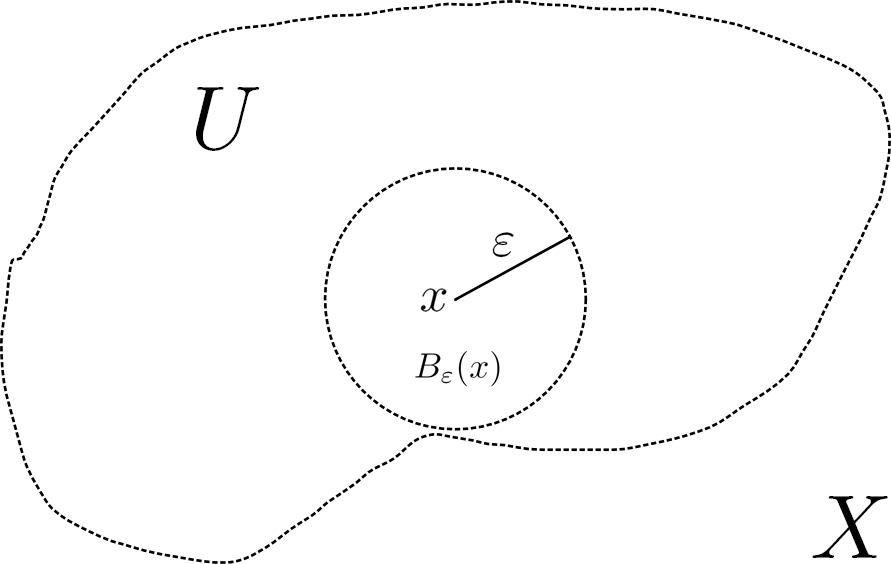
\includegraphics[width = .55\textwidth]{open_set}
		\caption{An open set $U$ in $\mathbb R^2$. At any point in the set, we can choose some $\epsilon$ small enough such that $B_\epsilon(x)\subseteq U$. In the picture, possible choices of $\epsilon$ for the points $x, y\in U$ are $\epsilon_1, \epsilon_2$. Pictorially, the balls of these radii centered around $x$ and $y$ are denoted by the dashed green circles. Note that we do not include the boundary in the definition of $U$ (i.e. we draw $U$ with dashed lines, which means it does not contain the bounding curve). If we include the boundary, $U$ is no longer an open set, because boundary points are not interior points: at a boundary point $p$, for each $\epsilon > 0$ the ball $B_\epsilon(p)$ does not lie completely inside $U$, no matter how small $\epsilon$ is! Draw a picture of this to convince yourself.}
		\label{fig:open_set}
	\end{figure}
	
	\begin{theorem}
	For any $x\in X$ and $\epsilon > 0$, the set $B_\epsilon(x)$ is open. Similarly, $\overline B_\epsilon(x)$ is closed.
	\end{theorem}
	
	\begin{proof} Exercise. \end{proof}
	
	Now for the important part; these next theorems will give us some ideas behind the axioms of topology, and we will use it in topology to classify open sets. 
	We begin with an obvious one:
	
	\begin{theorem}
		The sets $X$ and $\emptyset$ are both open (and hence closed) in any metric space $X$.
	\end{theorem}
	
	\begin{proof} 
		For any $x\in X$, the set $B_1(x)\subseteq X$, so we are done.
	\end{proof}
	
	These next two theorems will show us how to create new open sets out of existing collections of open sets. Later, we will develop these into axioms for 
	a topology, and so understanding them is quite important.
	
	\begin{theorem}
	Let $\{U_\alpha\}_{\alpha\in A}$ be an arbitrary collection of open sets. Then
	\begin{equation}
		\bigcup_\alpha U_\alpha
	\end{equation}
	is open.
	\end{theorem}
	
	\begin{proof}
		Take $x\in \cup_\alpha U_\alpha$. Then for some $\alpha\in A$, $x\in U_\alpha$, so there exists $\epsilon > 0$ such that $B_\epsilon(x)\subseteq 
		U_\alpha\subseteq \cup_\alpha U_\alpha$, and hence $x$ is an interior point and $\cup_\alpha U_\alpha$ is open.
	\end{proof}
	
	\begin{theorem}
	Let $\{U_i\}_{i = 1}^n$ be a finite collection of open sets. Then 
	\begin{equation}
		\bigcap_{i = 1}^n U_i
	\end{equation}
	is open.
	\end{theorem}
	
	\begin{proof}
		Pick $x\in\cap_\alpha U_\alpha$. Then for each $i = 1, ..., n$, $x\in U_i$, so there exists $\epsilon_i$ such that $B_{\epsilon_i}(x)\subseteq U_i$. Take 
		$\epsilon := \min \{\epsilon_1, ..., \epsilon_n\}$, and then $B_\epsilon(x)\subseteq B_{\epsilon_i}(x)\subseteq U_i$ for each i, so:
		\eq
			B_\epsilon(x)\subseteq\, \bigcap_\alpha U_\alpha
		\qe
		and thus $\cap_\alpha U_\alpha$ is open.
	\end{proof}
	
	These two conditions look quite similar, but they are really quite different; the first asserts that open sets are closed under \textbf{arbitrary} unions, including 
	infinite unions, while the second only states that open sets are closed under finite intersections. These can be quite different in practice, as for example if 
	we have a collection of open sets $A := \{U_x : x\in (0, 1)\}$ we know that $\cup A$ is an open set, but we do not know if $\cap A$ is open because the 
	indexing set is finite. Note the immediate corollary for closed sets:
	
	\begin{corollary}
		The finite union of closed sets is closed, and the arbitrary union of closed sets is closed.
	\end{corollary}
	
	\begin{proof}
		Just apply DeMorgan's laws:
		\begin{align}
			\left(\bigcup_\alpha U_\alpha \right)^c = \bigcap_\alpha U_\alpha^c &&
			\left(\bigcap_\alpha U_\alpha \right)^c = \bigcup_\alpha U_\alpha^c.
		\end{align}
	\end{proof}

\newpage
\section{Limit Points}

	Limit points generalize the notion of the limit of a sequence in $\mathbb R^n$. Of course, we must start with defining a sequence, as well as what it means for a sequence to converge. Your intuition on sequences in $\mathbb R$ should help you here; a sequence converges if its points eventually get arbitrarily close together. More precisely, we have the following definition.
	
	\begin{definition}[Sequence, Convergence]
	A \textbf{sequence} in $X$ is a map $x : \mathbb N\rightarrow X$. As notation, we write $x_n$ for $x(n)$, and denote the entire sequence by $(x_n)$.
	\newline\newline
	Let $(x_n)$ be a sequence in $X$. We say that $(x_n)$ \textbf{converges} to $x_0\in X$ if for every $\epsilon > 0$, there exists $N\in\mathbb N$ such that $\forall n\geq N$, $d(x_n, x_0) < \epsilon$. If $(x_n)$ converges to $x_0$, we write $(x_n)\rightarrow x_0$ or $\lim x_n = x_0$.
	\end{definition}
	
	This definition is just a reformulation of what we think convergence means on $\mathbb R$. If $x_n\rightarrow x_0$, then for every small tolerance $\epsilon
	$ around $x_0$, we may go far enough in the sequence (that is what $N$ is) so that we stay within $\epsilon$ of $x_0$. It would be no good if we only 
	needed to find a point in the sequence within $\epsilon$ of $x_0$, for then a sequence that alternates between $0$ and $1$ would converge to $0$ and 
	$1$. Instead, we require that we must find $N$ such that every $n\geq N$ has $x_n$ within this tolerance, so that the sequence stays equally close 
	to its limit. There is also another type of sequence that we will study, called a Cauchy sequence. These are sequences which eventually get arbitrarily close, 
	but need not converge. 
	
	\begin{definition}[Cauchy Sequence]
		Let $(x_n)$ be a sequence in $X$. We say that $(x_n)$ is a \textbf{Cauchy sequence} if for each $\epsilon > 0$, there is $N\in\mathbb N$ such that 
		$\forall n, m\geq N$, $d(x_n, x_m) < \epsilon$.
	\end{definition}
	
	In $\mathbb R$, every Cauchy sequence converges, so you will not find any examples here of a non-convergent Cauchy sequence. 
	You will need to look at a different example of a metric space like $\mathbb Q$ to find an example of a Cauchy sequence which doesn't converge; pick a 
	sequence in the rational numbers which would converge to $\sqrt{2}$. This does not converge in $\mathbb Q$, so we can see by example that not every 
	Cauchy sequence in $\mathbb Q$ converges. Note that in any metric space, any convergent sequence is Cauchy. Now, let's switch gears a bit; we will generalize 
	the notion of a limit to something called a limit point.
	
	\begin{definition}[Limit Point]
		Let $A\subseteq X$ be a subset of a metric space. We call $x\in X$ a \textbf{limit point} of $A$ if for every $\epsilon > 0$, we have:
		\eq
			A\cap(B_\epsilon(x)\setminus\{x\})\neq\emptyset.
		\qe
	\end{definition}
	
	In other words, $x$ is a limit point if no matter how small a neighborhood we take around $x$, we can always find a point of $A$ (which is \textbf{not} $x$, 
	hence why we subtracted $\{x\}$ in the definition) contained in this neighborhood. To see why this generalizes the notion of a limit, we have a theorem:
	
	\begin{theorem}
		Let $A\subseteq X$, and $x\in X$. Then $x$ is a limit point of $A$ iff there is a sequence $(x_n)_{n\in\mathbb N}$ with values in $A$ such that:
		\eq
			x = \lim x_n.
		\qe
	\end{theorem}
	
	\begin{proof}
		We prove the forward direction; suppose that $x$ is a limit point. Then for each $n\in\mathbb N$, let $\epsilon_n := \frac{1}{n} > 0$. By the definition of 
		a limit point, this implies that
		\eq
			A\cap(B_{\epsilon_n}(x)\setminus\{x\})\neq\emptyset.
		\qe
		Pick $x_n$ to be an element in this nonempty set. Then $d(x, x_n) < \epsilon_n = \frac{1}{n}$, and so $(x_n)$ converges to $x$.
	\end{proof}
	
	The converse of this will be an exercise. Limit points also have a close connection to closed sets-- for these definitions/theorems, let $A\subseteq X$ be 
	a subset of $X$.
	
	\begin{definition}[Closure]
		The \textbf{closure} of $A$ is the set:
		\eq
			\overline A := A\cup\{x\in X : x\textnormal{ is a limit point of $A$}\}.
		\qe
	\end{definition}
	
	Now for a couple theorems to explain the importance of the notion of closure.
	
	\begin{theorem}
		$A$ is closed if and only if it contains all its limit points, i.e. $A= \overline{A}$.
	\end{theorem}
	
	\begin{proof}
		Recall $A$ is closed if its complement is open. Suppose that $A$ is closed, so $A^c$ is open. Obviously $A\subseteq\overline A$, so we show the 
		reverse inclusion. Suppose $x$ is a limit point of $A$ not in $A$. Then $x	\in A^c$, so there is an open ball of radius $\epsilon > 0$ centered at $x$ 
		contained in $A^c$. But then:
		\eq
			A\cap(B_\epsilon(x)\setminus\{x\}) = \emptyset
		\qe
		which contradicts that $x$ is a limit point. Thus $x\in A$, and so $A = \overline A$. You can do the converse, if you wish.
	\end{proof}
	
	\begin{theorem}
		The closure of $A$ of $A$ is a closed set, and is in fact the smallest closed set containing $A$ (i.e. if $A\subseteq B$ with $B$ closed, then $B$ must 
		contain $\overline A$ as well).
	\end{theorem}
	
	\begin{proof}
		I will sketch the proof: to show $\overline A$ is closed, show that $\overline{\overline A} = \overline A$. This may seem obvious, but it is not trivial. It 
		will reduce down to showing that every limit point of $\overline A$ is contained in $\overline A$. You can do this by showing that any limit point of 
		$\overline A$ is a limit point of $A$. To show that any closed set contains $\overline A$, this follows because any closed set containing $A$ must 
		contain all the limit points of $A$, and hence must contain $\overline A$. 
	\end{proof}
	
	The next definition generalizes how the rational numbers are embedded in $\mathbb R$. In particular, $\mathbb Q$ is \textbf{dense} in $\mathbb R$, which 
	means that given any two real numbers $r_1\neq r_2$ (arbitrarily close, but never equal), we can find a rational number $q\in (r_1, r_2)$. 
	
	\begin{definition}[Dense Set]
		Let $X$ be a metric space, and $S\subseteq X$. We say that $S$ is \textbf{dense} in $X$ if $\overline{S} = X$. 
	\end{definition}
	
	So, a subset $S$ of a metric space $X$ is dense if every point in $X$ is a limit point of $S$. No matter how small we make an $\epsilon$-ball, we will always 
	have some members of a dense subset contained in the ball.
	
\newpage
\section{Functions on Metric Spaces}

	\subsection{Continuity}

	Continuity is a property of maps that you've probably dealt with for quite a long time; for maps $f : \mathbb R\rightarrow\mathbb R$, the notion of continuity 
	is equivalent to tracing a finger along the graph of $f$ without having to lift it up. To be more precise:
	
	\begin{definition}[Continuity in $\mathbb R$]
		Let $f : \mathbb A\subset\mathbb R\rightarrow \mathbb R$ be a map, and let $x_0\in A$. We say that $f$ is \textbf{continuous at $x_0$} if for every 
		$\epsilon > 0$, there exists $\delta > 0$ such that $|x - x_0| < \delta\implies |f(x) - f(x_0)| < \epsilon$. A function $f$ is \textbf{continuous on $A$} if 
		it is continuous at every point in $A$. If $A = \mathbb R$, we say $f$ is a \textbf{continuous function}.
	\end{definition}
	
	Intuitively, this means that no matter how close we get to $f(x_0)$, we can always find a neighborhood around $x$ that maps at least this close to $f(x_0)$. 
	Try to visualize what this means for a discontinuous function; consider the Heaviside step function $\Theta(x)$, which is unity for $x \geq 0$ and zero for $x
	< 0$. $\Theta(x)$ is not continuous at $0$; take $\epsilon = \frac{1}{2}$. Then no matter how small I pick $\delta$, $\Theta(-\frac{\delta}{2}) = 0$ because it 
	is negative, and this is not within $\epsilon$ of $f(0) = 1$. We see that in this case, the definition agrees with our intuition.
	
	Let's try to formulate this in the language of metric spaces. In the above definition, we were using the standard metric on $\mathbb R$ induced by the 
	$|\cdot|$ function. Another way to say this definition is that given any $\epsilon$ ball around $f(x_0)$, we can find a $\delta$ ball around $x_0$ that is 
	mapped by $f$ into the $\epsilon$ ball. This will be our definition of continuity on metric spaces.
	
	\begin{definition}[Continuity]
		Let $f : X\rightarrow Y$ be a map between metric spaces, and let $x_0\in X$. Then $f$ is \textbf{continuous at $x_0$} if for every $\epsilon > 0$, there 
		exists $\delta > 0$ such that:
		\eq
			f(B_\delta(x_0))\subseteq B_\epsilon(f(x_0)).
		\qe
	\end{definition}
	
	And the usual notions of $f$ being continuous on a set or on $X$ are the same as before when we considered functions in $\mathbb R$. Let's unpack this 
	definition; suppose $f$ is continuous at a point $x_0$. The $\forall\epsilon > 0$, $\exists\delta > 0$ such that $f(B_\delta(x_0))\subseteq B_\epsilon(f(x_0))$. 
	What does this mean? It is exactly what we stated above for $\mathbb R$; if $d(x, x_0) < \delta$, then $x\in B_\delta(x_0)$ and so $f(x)\in f(B_\delta(x_0))
	\subseteq B_\epsilon(f(x_0))$. Because $f(x)\in B_\epsilon(x_0)$, we have
	\eq
		d(f(x), f(x_0)) < \epsilon.
	\qe
	And we see that we have an equivalent definition of continuity; $\forall\epsilon > 0$, $\exists\delta > 0$ such that $d(x, x_0) < \delta\implies d(f(x), f(x_0)) < 
	\epsilon$. This is the definition we made above in the case of $\mathbb R$, and we see that we have successfully generalized the definition.
	
	Now we state the theorem that motivates how we define continuity on an arbitrary topological space. The proof is pretty fun to do yourself, so I would 
	encourage you to try it out, and let me know if you need any help with it. Here is the theorem:
	
	\begin{theorem}
		Let $f : X\rightarrow Y$ be a map between metric spaces. The following are equivalent.
		\begin{enumerate}
			\item $f$ is continuous.
			\item Given any sequence $(x_n)$ in $X$ converging to $x_0$, we have:
			\eq
				\lim f(x_n) = f(x_0).
			\qe
			\item $f$ pulls back open sets into open sets, i.e. for every open set $V\subseteq Y$, 
			\eq
				f^{-1}(V)
			\qe
			is open in $X$.
		\end{enumerate}
	\end{theorem}
	
	The 3rd statement is the one we are interested in and will generalize in topology, because it deals with how $f$ treats open sets. Specifically, the preimage 
	of an open set under a continuous map is open, and we will see exactly how powerful of a notion this is later.
	
	\subsection{Uniform Continuity}
	
	Continuity is a nice property for a function to have, but we can actually ask for a function to satisfy a stronger property. Suppose a function $f$ is continuous.  
	Then if I give you an $\epsilon > 0$, then for every $x$, you can find a $\delta > 0$ such that $f$ maps the $\delta$-ball around $x$ into the $\epsilon$-ball 
	around $f(x)$. However, note that this $\delta$ \textit{depends on $x$}; in other words, $\delta = \delta_x$, and $\delta$ can change if you consider a different 
	$x$. The idea behind uniform continuity is to classify functions which are ``nicer" than continuous functions in this sense. If you are given a uniformly 
	continuous function, you can find a $\delta > 0$ that makes the $\delta$-ball around $x$ map into the $\epsilon$ ball around $f(x)$ \textit{for any $x\in X$}. 
	
	\begin{definition}[Uniform Continuity]
		Let $f : X\rightarrow Y$ be a map between metric spaces. We say $f$ is \textbf{uniformly continuous} if for all $\epsilon > 0$, there exists $\delta > 0$ 
		such that $d(x, y) < \delta$ implies $d(f(x), f(y)) < \epsilon$. 
	\end{definition}
	
	Just as continuous functions take convergent sequences into convergent sequences, uniformly continuous functions satisfy an even stronger property of 
	this. 
	
	\begin{prop}
		Let $f : X\rightarrow Y$ be uniformly continuous, and $(x_n)$ a Cauchy sequence in $X$. Then $(f(x_n))$ is a Cauchy sequence in $Y$. 
	\end{prop}
	
	\subsection{Isometries}
	
	Metric spaces form a category in the arrow-theoretic sense, so it is a natural question to ask what the morphisms of this category are. We will call the 
	morphisms \textbf{isometries}. To be precise:
	
	\begin{definition}[Isometry]
		Let $f : X\rightarrow Y$ be a map between metric spaces. We say $f$ is an \textbf{isometry} if $f$ preserves the metric, i.e. for each $x_1, x_2
		\in X$, we have:
		\eq
			d(f(x_1), f(x_2)) = d(x_1, x_2).
		\qe
		If $f$ is surjective, then we will view $f$ as a \textbf{metric space isomorphism}.
	\end{definition}
	
	\begin{prop}
		If $f : X\rightarrow Y$ is an isometry of metric spaces, then $f$ is an injection.
	\end{prop}
	
	If $f$ is a surjective isometry, we call it \textbf{isometric onto}. Note that if $f$ is isometric onto, then $f^{-1}$ is as well, because $f$ will be a bijection and 
	$f^{-1}$ will be an isometry.
	
	\subsection{Lipschitz Functions}
	
	Here is the final type of function between metric spaces we will be interested in. In $\mathbb R$, these functions look similar to differentiable functions, but 
	we can define them in a more general setting.
	
	\begin{definition}[Lipschitz]
		Let $f : X\rightarrow Y$ be a map between metric spaces. We say that $f$ is \textbf{Lipschitz} if there exists a constant $k_f\in\mathbb R$ such that:
		\eq
			d(f(x_1), f(x_2)) \leq k_f d(x_1, x_2)
		\qe
		for each $x_1, x_2\in X$. If $f$ is Lipschitz, then the smallest such $k_f$ that satisfies this condition is called the \textbf{Lipschitz constant} of $f$, denoted 
		$L(f)$.
	\end{definition}
	
	\begin{prop}
		Any Lipschitz function is uniformly continuous.
	\end{prop}

\newpage	
\section{Completions}

	Let $(X, d)$ be a metric space. One important property of metric spaces that we will now study is \textbf{completeness}. This property is very important, and is 
	one of the properties that makes $\mathbb R$ a ``nicer" metric space than $\mathbb Q$. The idea is that $\mathbb R$ has no ``holes" in it; even though 
	$\mathbb Q$ is dense in $\mathbb R$, $\mathbb Q$ still has an infinite number of holes. Intuitively, $\mathbb R$ is given from $\mathbb Q$ by adding in all the 
	holes between rational numbers. The goal of this section of notes is to make this notion precise, and to extend it to arbitrary metric spaces. 
	
	\begin{definition}[Complete Space]
		We say that $(X, d)$ is \textbf{complete} if every Cauchy sequence in $X$ converges.
	\end{definition}
	
	So, $\mathbb Q$ is not a complete metric space, but $\mathbb R$ is. It turns out that $\mathbb R$ is the only complete metric space that we can isometrically 
	embed $\mathbb Q$ into. This begs the question: given a metric space $X$, can we find a complete metric space and an isometric embedding of $X$ into 
	this space? The answer is yes, and we will call this space a \textbf{completion} of $X$.
	
	\begin{definition}[Completion]
		Let $(X, d)$ be a metric space. By a \textbf{completion} of $X$ we mean a complete metric space $\tilde X$ together with an isometric function $f : X
		\rightarrow\tilde X$ such that $\im(f)\subseteq\tilde X$ is dense.
	\end{definition}
	
	\begin{prop}
		Let $((\tilde X, d), j_X)$ and $(( Z, d'), j_Z)$ be two completions of $X$. Then $\exists !\phi : \tilde X\rightarrow Z$ isometric onto such that $j_z = 
		\phi\circ j_X$, i.e. the following diagram commutes:
		\[
		\begin{tikzcd}
			X \arrow[r, "j_X"] \arrow[rd, bend right, "j_Z"] & \tilde X \arrow[d, "\phi"] \\
			& Z
		\end{tikzcd}
		\]
	\end{prop}
	
	So, the completion of a metric space is unique up to isometry. Now, we will show that there is a natural way to extend a map from a dense subspace of a 
	metric space to the space itself. As an example of this, if I define a uniformly continuous function on $\mathbb Q$ into a complete metric space, one can 
	construct a continuous extension of this map to $\mathbb R$, the completion of $\mathbb Q$. 
	
	\begin{prop}
		Let $X, Y$ be metric spaces with $Y$ complete. Let $S$ be a dense subset of $X$ equipped with the subspace metric. Let $f : S\rightarrow Y$ be 
		uniformly continuous. Then $\exists ! \overline f : X\rightarrow Y$ such that $\overline f$ is an extension of $f$ to $X$ (i.e. $\overline f|_S = f$) and 
		$\overline f$ is uniformly continuous.
	\end{prop}
	
	\begin{proof}
		We will construct such a $\overline f$. Let $x\in X\setminus S$. Pick a sequence $(s_n)$ such that $s_n\rightarrow x$, which we may find because 
		$S$ is dense in $X$. Then, define:
		\eq
			\overline f(x) := \lim f(s_n).
		\qe
		Note that this is well defined because $(f(s_n))$ is a Cauchy sequence as $f$ is uniformly continuous and $(s_n)$ is Cauchy in $X$; then as $Y$ is 
		complete, this limit exists. We will show that this is well defined, so let $(t_n)$ be another Cauchy sequence in $S$ converging to $x$. We will show 
		that $\lim s_n = \lim t_n$. Because $s_n, t_n\rightarrow x$, $d(s_n, t_n)\rightarrow 0$ as $n\rightarrow\infty$. But, $f$ is uniformly continuous, so we 
		also have $d(f(s_n), f(t_n))\rightarrow 0$ as $n\rightarrow\infty$, which implies that $\lim f(t_n) = \lim f(s_n)$, hence the map $\overline f$ is well 
		defined.
	\end{proof}
	
	\begin{definition}
		For any metric space $(X, d)$, let $\mathrm{Cau}(X)$ be the set of all Cauchy sequences in $X$. Let $(s_n), (t_n)\in \mathrm{Cau}(X)$. We say that $(s_n)$ and $(t_n)$ are \textbf{equivalent} if $d(s_n, t_n)\rightarrow 0$ as $n\rightarrow\infty$. 
	\end{definition}
	
	Now, we will explicitly construct a completion for an arbitrary metric space using this notion of equivalence of Cauchy sequences. We will quotient $\mathrm{Cau}(X)$ out by this relation to form a complete space that $X$ naturally embeds into. So, our goal is to prove the following theorem.
	
	\begin{theorem}
		Every metric space has a completion.
	\end{theorem}
	
	\subsection{Proof: Construction of the Completion}
	
	Let $(X, d)$ be a metric space. To prove the theorem above, we begin with a lemma.
	
	\begin{lemma}
		The relation $(s_n)\sim (t_n)$ iff $(s_n)$ and $(t_n)$ are equivalent is an equivalence relation on $\mathrm{Cau}(X)$.
	\end{lemma}
	
	This is quite easy to show, and follows almost immediately from the definition. So, define:
	\begin{align}
		\tilde X := \mathrm{Cau}(X) / \sim && j : X\hookrightarrow\tilde X, x\mapsto (x_n)\; \mathrm{mod}\, \sim.
	\end{align}
	We have defined a new space $\tilde X$ and an embedding $j$ of $X$ into $\tilde X$. Now, we need to put a metric $\tilde d$ on 
	$\tilde X$ which makes $j$ an isometry.
	
	\begin{prop}
		Let $\tilde X = \mathrm{Cau}(X)/\sim$ as above, and let $\xi, \eta\in \tilde X$. Pick representatives $(x_n), (y_n)\in\xi, \eta$. Then, the map:
		\eq
			\tilde d(\xi, \eta) := \lim d(x_n, y_n)
		\qe
		defines a metric on $\tilde d$.
	\end{prop}
	
	To show this indeed defines a metric, we first need to show it is well defined. So, let $(x_n'), (y_n')\in\xi, \eta$ be other representatives. Then $\lim d(x_n, x_n') 
	= 0$ and $\lim d(y_n, y_n') = 0$, and we need to show that $\lim d(x_n, y_n) = \lim d(x_n', y_n')$. This will follow from an $\frac{\epsilon}{3}$ argument. The 
	other properties of a metric should follow relatively easily from the definition of $\tilde d$ and the fact that $d$ is a metric. Now, 
	note that
	\eq
		\tilde d(j(x), j(y)) = \lim d(x, y) = d(x, y).
	\qe
	So we indeed have an isometry. Finally, we need to show that $j(X)\subseteq\tilde X$ is dense. Let $\xi\in\tilde X$ and let $\epsilon > 0$. Let $(x_n)\in\xi$ be a 
	representative. Choose $N\in\mathbb N$ such that $n, m\geq N\implies d(x_n, x_m) < \frac{\epsilon}{2}$. Consider $j(x_N)$. Then we have
	\eq
		\tilde d(j(x_N), \xi) = \lim_{n\rightarrow\infty} d(x_N, x_n) \leq \frac{\epsilon}{2} < \epsilon.
	\qe
	Note that to be precise, we needed to pick $\frac{\epsilon}{2}$ because a limit of numbers which are strictly less than another number $a$ can still be equal to 
	$a$. So, this shows that $j(X)\subseteq\tilde X$ is dense. The final thing to show is that $(\tilde X, \tilde d)$ is a complete metric space. Let $(\xi_n)$ be a 
	Cauchy sequence in $\tilde X$. For each $m\in\mathbb N$ choose $x_m$ such that $\tilde d(j(x_m), \xi_m) < \frac{1}{m}$ (we may do this by the density of $X$ 
	in $\tilde X$). Then, one can check that $(x_m)$ is Cauchy in $X$, and $(\xi_n)\rightarrow\eta$, where $\eta$ is the equivalence class of $(x_m)$ in $\tilde X$.
	This completes the construction!
	
	\subsection{Completion of a Vector Space}
	
	Let $V$ be a vector space with norm $||\cdot||$. We can add and scale Cauchy sequences in $\Cau(V)$ pointwise, so $\Cau(V)$ is a vector space itself. 
	Let $N(V)$ be the sequence of Cauchy sequences converging to $0$ in $V$. This is a subspace of $\Cau(V)$. Note that if $(v_n)\sim (w_n)$, then $||v_n - 
	w_n||\rightarrow 0$, and so $(v_n - w_n)\in N(V)$. The converse follows as well. So, the completion of $\Cau(V)$ forces all of these equivalent Cauchy 
	sequences to be identical, and therefore it is
	\eq
		\tilde V = \Cau(V) / N(V).
	\qe
	In particular, this means that the completion of a vector space is complete vector space.

\newpage
\section{Examples}

	We now examine some examples of metric spaces that we will often run into. First, suppose that we have a vector space $V$.
	
	\begin{definition}[Norm]
		Let $V$ be a vector space over $\mathbb F = \mathbb R$ or $\mathbb F = \mathbb C$. By a \textbf{norm} on $V$, we mean a function $||\cdot|| : V
		\rightarrow\mathbb R^+$ such that:
		\begin{enumerate}
			\item For $z\in\mathbb F$, $v\in V$, we have $||zv|| = |z|\cdot||v||$.
			\item For $v, w\in V$, we have $||v + w||\leq ||v|| + ||w|$.
			\item For $v\in V$, we have $||v|| = 0$ iff $v = 0\in V$.
		\end{enumerate}
	\end{definition}
	
	Norms are generalizations of lengths of vectors. Any inner product $\langle\cdot, \cdot\rangle$ on $V$ induces a canonical metric $||v|| = \langle v, v
	\rangle^{\frac{1}{2}}$. In $\mathbb R^n$, the standard inner product will just induce the Euclidean norm of a vector. Over the vector spaces $\mathbb R^n$ or $
	\mathbb C^n$, we can actually generalize the Euclidean norm a bit with the notion of a $p$-norm.
	
	\begin{prop}
		Let $V = \mathbb R^n$ or $\mathbb C^n$. Then for $p\in\mathbb N$, we can define a norm by
		\eq
			||v||_p := (\sum_{i = 1}^n |v_i|^p)^{\frac{1}{p}},
		\qe
		and we can also define
		\eq
			||v||_\infty := \sup_j\{|v_j|\}.
		\qe
		The first norm is called the \textbf{$p$-norm}, and the second norm is the \textbf{sup norm}.
	\end{prop}
	
	The $p$-norm often finds applications in other fields like computer science and engineering. As lengths give rise to distances, the next theorem should be no 
	surprise.
	
	\begin{theorem}
		Let $V$ be a vector space with norm $||\cdot||$. Then, $V$ is a metric space under metric:
		\eq
			d(v, w) = ||v - w||.
		\qe
	\end{theorem}
	
	So, any normed vector space is a metric space, which generates a lot of examples of metric spaces for us. One important examples is $C([0, 1])$ (for 
	any topological space, $C(X)$ is the space of continuous functions $f : X\rightarrow\mathbb R$). Here are some examples of norms that we can put on 
	$C([0, 1])$, which we will see quite often. 
	\begin{itemize}
		\item The \textbf{$p$-norm}. For $f\in C([0, 1])$, this is:
		\eq
			||f||_p := \left(\int_0^1|f(x)|^p dx\right)^{\frac{1}{p}}.
		\qe
		\item The \textbf{uniform norm}. For $f\in C([0, 1])$, this is:
		\eq
			||f||_\infty := \sup_{x\in [0, 1]} \{|f(x)|\}.
		\qe
	\end{itemize}
	An important proposition we will use is the following.
	\begin{prop}
		The space $C([0, 1])$ under the uniform norm is complete.
	\end{prop}
	However, note that the property of being complete does depend on the metric you are using. The same space $C([0, 1])$ is not complete under either the 
	1-norm or the 2-norm. For example, consider the sequence of functions $(f_n)$ in $C([0, 1])$ given by:
	\eq
		f_n(x) := \begin{cases}
			1 & x\leq\frac{1}{2} \\
			1 - n(x - \frac{1}{2}) & \frac{1}{2}\leq x \leq\frac{1}{2} + \frac{1}{n} \\
			0 & \frac{1}{2} + \frac{1}{n} \leq x
		\end{cases}.
	\qe
	This sequence is Cauchy under the 1-norm, but not under the uniform norm. To visualize the uniform norm intuitively, the best way to think of an $\epsilon$-ball 
	with respect to $||\cdot||_\infty$ as an $\epsilon$-tube, as in Fig.~\eqref{fig:eps_tube}. That is, two functions $f$ and $g$ have $||f - g||_\infty < \epsilon$ iff $|f(x) - g(x)| < \epsilon$ for each $x\in [0, 1]$, so they lie in the same $\epsilon$-tube.
	
	\begin{figure}[!htp]
		\centering
		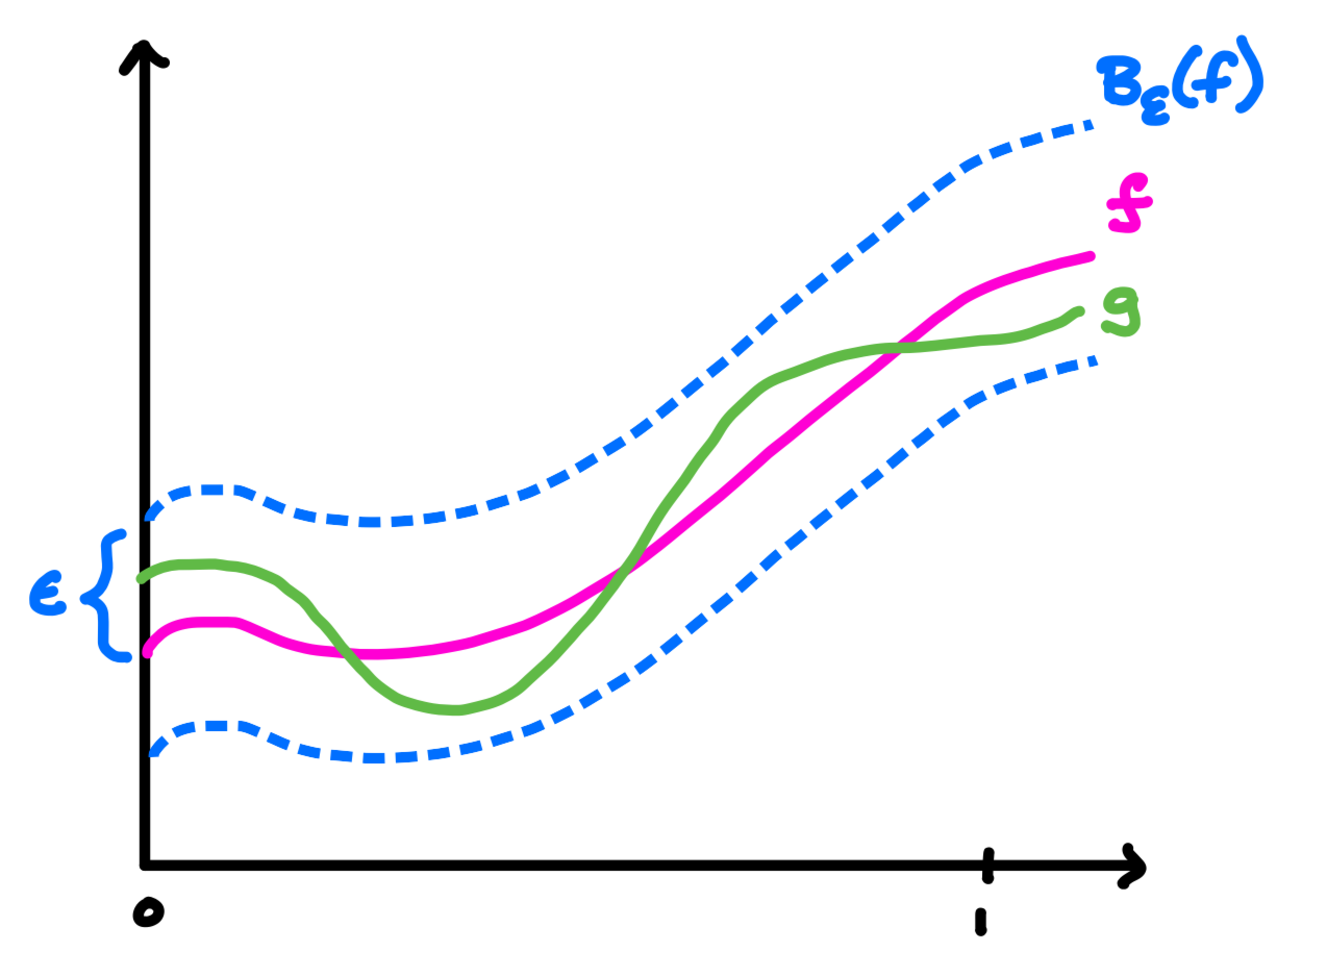
\includegraphics[width = 0.7\textwidth]{epsilon_tube}
		\caption{Visualization of the $\epsilon$-tube around the pink function $f$, $B_\epsilon(f) := \{h\in C([0, 1]) : ||f - h||_\infty < \epsilon\}$. Intuitively, $B_\epsilon(f)$ is a tube of radius $\epsilon$ centered at $f$, given in the diagram by the blue dashed lines. Any function, for example the green function $g$, that lies within the two dashed lines is in $B_\epsilon(f)$, hence $g\in B_\epsilon(f)$. The uniform norm creates the tube because we consider the $\sup$ over $x\in [0, 1]$ of the maximum deviation from $x$; hence one way to think about $B_\epsilon(f)$ is as the space of all functions whose maximum deviation from $f$ at any point $x\in [0, 1]$ is $< \epsilon$.}
		\label{fig:eps_tube}
	\end{figure}
	

\end{document}